\subsection{Propeller Aerodynamics}
Aerodynamics are assumed to be faster than mechanical dynamics of the actuator.
The thrust generation process due to the propagation of pressure wave is assumed to be instantaneous. This assumption is inherent to the standard models that use potential flow theory (lifting-line, blade-element and momentum-disk theories), as they assume incompressible flow.\\

\itbf{Propeller Thrust}:
\begin{align*}
    F_T = C_{T} \omega^2
\end{align*}

\itbf{Propeller moment due to drag}:
\begin{align*}
    M_D = C_{D} \omega^2
\end{align*}

\textbf{Aeroelasticity of the propeller:} It is assumed that the aeroelasticity of the propeller produces high-frequency oscillations in the thrust and torque of the propller which are assumed to be very fast and roll off w.r.t the mechanical dyanmics dyanmics of the actuator as well as the transmission through the propller shaft. The constant  bias in the torque due to flutter is captured in the drag coefficient and it's parameter uncertainity.\\

In the experimental setup, the total moment measured is the result of aerodynamic moment and the friction of the BLDC motor. Thus the total moment becomes:
\begin{align*}
    M = C_D \omega^2 + b_f \omega + M_f
\end{align*}

The aerodynamic coefficients are estimated from the static measuremnts using least-squares estimation.

\begin{align*}
    C_T &= 7.1e-6 \, {N.s^2/rad^2}\\
    C_D &= 2.5e-8 \, {Nm.s^2/rad^2}\\
    b_f &= 9.3e-6 \, {Nm.s/rad}\\
    M_f &= 5.8e-7  \, {Nm}
\end{align*}

\begin{figure}[H]
    \begin{minipage}{0.49\textwidth}
        \begin{figure}[H]
            \centering
            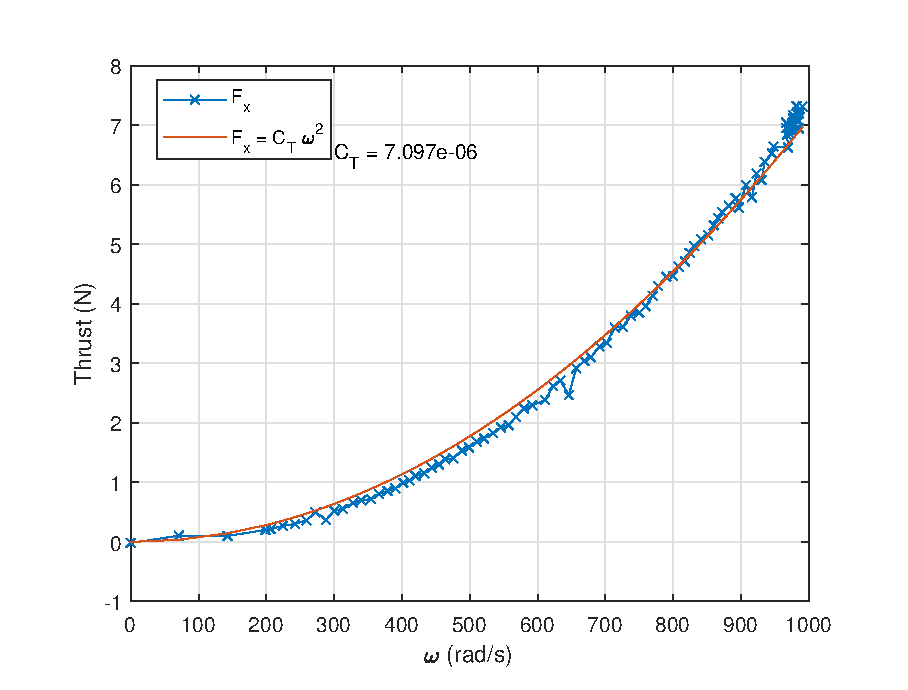
\includegraphics[width = \textwidth]{./figs/aero/Fx.eps}
        \end{figure}
        \caption{Variation of thrust with rpm}
    \end{minipage}
    \begin{minipage}{0.49\textwidth}
        \begin{figure}[H]
            \centering
            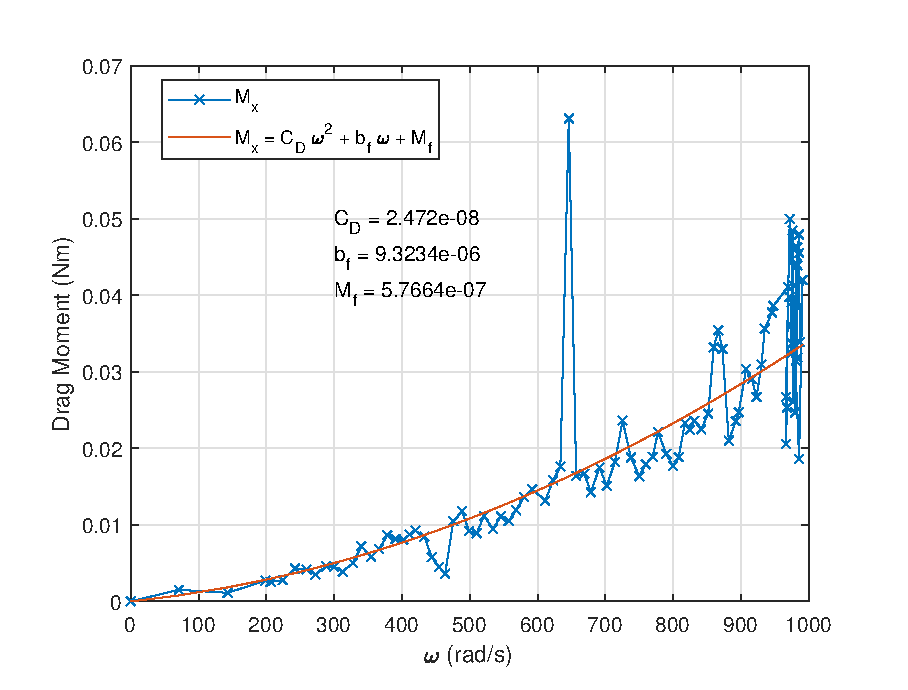
\includegraphics[width = \textwidth]{./figs/aero/Mx.eps}
            \caption{Variation of drag moment with rpm}
        \end{figure}
    \end{minipage}
\end{figure}
